\documentclass[11pt
              , a4paper
              , twoside
              , openright
              ]{report}


\usepackage{float} % lets you have non-floating floats

\usepackage{url} % for typesetting urls

% Personal Packages
\usepackage[utf8]{inputenc}
\DeclareUnicodeCharacter{2190}{$\leftarrow$}
\DeclareUnicodeCharacter{2192}{$\rightarrow$}
\DeclareUnicodeCharacter{00B7}{$\cdot$}
\DeclareUnicodeCharacter{00D7}{$\times$}
\DeclareUnicodeCharacter{2193}{$\downarrow$}
\usepackage{semantic} % Dunno what for? I think inference rules
\usepackage{amssymb}
\usepackage{bcprules}
\usepackage[nounderscore]{syntax} % This is for grammar rules
\usepackage{listings}
\usepackage{lipsum}
\usepackage{macros/macros}
\usepackage{tikz}
\usetikzlibrary{shapes.geometric, arrows, matrix, positioning}

\usepackage{xcolor}
\definecolor{codegreen}{rgb}{0,0.6,0}
\definecolor{codegray}{rgb}{0.5,0.5,0.5}
\definecolor{codepurple}{rgb}{0.58,0,0.82}
\definecolor{backcolour}{rgb}{0.95,0.95,0.92}
 
\lstdefinestyle{mystyle}{
    backgroundcolor=\color{backcolour},   
    commentstyle=\color{codegreen},
    keywordstyle=\color{magenta},
    numberstyle=\tiny\color{codegray},
    stringstyle=\color{codepurple},
    basicstyle=\ttfamily\footnotesize,
    breakatwhitespace=false,         
    breaklines=true,                 
    captionpos=b,                    
    keepspaces=true,                 
    numbers=left,                    
    numbersep=5pt,                  
    showspaces=false,                
    showstringspaces=false,
    showtabs=false,                  
    tabsize=2
}
\lstset{style=mystyle}


\usepackage[colorinlistoftodos,prependcaption]{todonotes}
\newcommandx{\unsure}[2][1=]{\todo[linecolor=red,backgroundcolor=red!25,bordercolor=red,#1]{#2}}
\newcommandx{\change}[2][1=]{\todo[linecolor=blue,backgroundcolor=blue!25,bordercolor=blue,#1]{#2}}
\newcommandx{\info}[2][1=]{\todo[linecolor=OliveGreen,backgroundcolor=OliveGreen!25,bordercolor=OliveGreen,#1]{#2}}
\newcommandx{\improvement}[2][1=]{\todo[linecolor=Plum,backgroundcolor=Plum!25,bordercolor=Plum,#1]{#2}}
\usepackage[framemethod=TikZ]{mdframed}

\graphicspath{ {./figures/} }

%
%  We don't want figures to float so we define
%
\newfloat{fig}{thp}{lof}[chapter]
\floatname{fig}{Figure}

%% These are standard LaTeX definitions for the document
%%                            
\title{A Fast Virtual Machine for Kihi}
\author{Callum Li}

%% This file can be used for creating a wide range of reports
%%  across various Schools
%%
%% Set up some things, mostly for the front page, for your specific document
\usepackage[image,ecs]{vuwproject}

% You should specifiy your supervisor here with
%     \supervisor{Firstname Lastname}
% use \supervisors if there is more than one supervisor
\supervisor{Michael Homer}
% Unless you've used the bschonscomp or mcompsci
%  options above use
%   \otherdegree{OTHER DEGREE OR DIPLOMA NAME}
% here to specify degree
\otherdegree{Bachelor of Engineering with Honours in Software Engineering}

% Comment this out if you want the date printed.
\date{}

\begin{document}

% Make the page numbering roman, until after the contents, etc.
\frontmatter

%%%%%%%%%%%%%%%%%%%%%%%%%%%%%%%%%%%%%%%%%%%%%%%%%%%%%%%

%%%%%%%%%%%%%%%%%%%%%%%%%%%%%%%%%%%%%%%%%%%%%%%%%%%%%%%

\begin{abstract}

    A great abstract here.
    
\end{abstract}

%%%%%%%%%%%%%%%%%%%%%%%%%%%%%%%%%%%%%%%%%%%%%%%%%%%%%%%

\maketitle

\chapter*{Acknowledgments} \label{C:ack} 
I'd like to acknowledge some people :).


\tableofcontents

% we want a list of the figures we defined
\listof{fig}{Figures}

%%%%%%%%%%%%%%%%%%%%%%%%%%%%%%%%%%%%%%%%%%%%%%%%%%%%%%%

\mainmatter

%%%%%%%%%%%%%%%%%%%%%%%%%%%%%%%%%%%%%%%%%%%%%%%%%%%%%%%

% individual chapters included here
\chapter{Introduction} \label{C:intro}
A principal concern of many programming languages is performance. The goal of this project is to address those concerns in the context of the Kihi programming language. Specifically, this project attempts to addresses those concerns by creating a performance focussed implementation of the language. This implementation, also referred to as the Kihi Runner, is distinguished by its performance focussed features, in particular an optimisation pipeline capable of dynamically constructing more efficient and compact representations of Kihi programs. How effective these optimisations are is the primary question this report attempts to answer.

Firstly however, the report begins with a treatment of surrounding background material in chapter \ref{C:background}. This most importantly includes a explanation of the Kihi language and its origins, with special attention paid to its raison d'être and unique characteristics. However, this material may be skipped by readers who are already familiar with the language. The follow chapter presents the brunt of this project's work. It describes the design and implementation of the Kihi Runner, illustrating the various features of the Kihi Runner. Most interestingly, this includes an explanation of the aforementioned optimisation pipeline. 

The report closes with an evaluation of the Kihi Runner,

\todo[inline]{evaluation paragraph TODO}

language created by Timothy Jones and Michael Homer \cite{jones2018practice}
\chapter{Background} \label{C:background}
This chapter aims to provide an understanding of the surrounding background material. In particular, this chapter explains the variety of concepts surrounding the Kihi programming language alongside an explanation of the language itself. This includes an introduction to the programming paradigms that inspired Kihi such as functional programming, concatenative programming, and compositional programming. This is followed by a thorough explanation of Kihi, examining topics such as its purpose, grammar, and evaluation methods.

\section{Related Programming Paradigms}
\subsection*{Imperative Programming}
The world of programming began with imperative programming languages. Imperative languages describe a program using a series of statements, each representing an operation for the computer to perform. For low level languages such as machine code and assembly, these statements can be an almost direct reflection of the actual computer's behaviour. However, writing programs in these languages quickly becomes impractical as the complexity of the application grows. Higher level languages, such as Java and C++, overcome this by providing higher level abstractions, such as objects and procedures. These features enable programmers to handle greater complexity by elevating the level of reasoning; in contrast to low level languages where a programmer must reason about even minute details.


\subsection*{Functional Programming}
\begin{figure}[htb]
    \centering
    \begin{lstlisting}[language=Java]
public class Main {
    public static int imperative_sum(List<Integer> xs) {
        int sum = 0;
        for (int x : xs) {
            sum += x;
        }
        return sum;
    }

    public static int functional_sum(List<Integer> xs) {
        if (xs.isEmpty()) {
            return 0;
        }

        return xs[0] + functional_sum(xs.sublist(1, xs.size()));
    }
}
\end{lstlisting}
    \caption{A imperative implementation of summation and a functional implementation of summation.}
    \label{fig:imperative_vs_functional_example}
\end{figure}

Standing in contrast to imperative programming is functional programming. In contrast to imperative programming languages which describe a program using a series of statements, functional programming languages describe a program as a series of function evaluations. A function represents a transformation. A function is called pure when the transformation has no side effects, meaning the function has no observable effects aside from emitting the output \cite{FunctionalProgrammingHaskellWiki2019}. In contrast, statements in imperative languages are often impure.

A commonly touted benefit of functional programming is referential transparency \cite{FunctionalProgrammingHaskellWiki2019} \cite{thompson2011haskell}. Put simply, this means the result any particular function evaluation will always yield the same result. This benefit relies on the concept of pure functions but enables programs to be understood through simple reasoning about local state. This stands in contrast to imperative programs which often require using non-local deductive reasoning. Some people view this as further elevating the level of reasoning \cite{thompson2011haskell}.

% Figure \ref{fig:referential_transparency_example} illustrates the deductive reasoning required to understand typical Java code. 

In order to be considered a functional language, the language must provide first-class functions, which are functions that can be treated as values. Java 8+ provides this in the form of lambda expressions, allowing for programs to written in a functional manner. An example of this is shown in figure \ref{fig:imperative_vs_functional_example}. Colloquially however, Java and languages like it are not considered functional programming languages because the predominant paradigm is not functional programming, rather it is object orientation or some other paradigm respectively.


\subsection*{Concatenative and compositional languages} 
Compositional and concatenative are two labels that are often used in tandem when describing a programming language. The former describes a language where the main interaction is function composition as opposed to function application. Figure \ref{fig:applicative_vs_compositional_example} demonstrates this difference by comparing how each paradigm interprets \lstinline{f g x}. The label concatenative is used to describe a language where the source code of two programs can be meaningfully concatenated together. These two labels are often found together because concatenative languages naturally encourage a compositional approach to programming because it allows for programs to understood as pipelines. In contrast, an applicative concatenative language has no such simple mental model.

\begin{figure}[!htb]
    \centering
    \begin{lstlisting}
Applicative (e.g. Haskell):
    f g x = (f(g))(x) 

Compositional (e.g. Forth):
    f g x = f(g(x))
\end{lstlisting}
    \caption{A demonstration of the differences between an applicative and compositional language.}
    \label{fig:applicative_vs_compositional_example}
\end{figure}

\begin{figure}[htb]
    \centering
    \begin{lstlisting}[language=Forth]
: STACK-EMPTY DEPTH 1 = ;

: SUM BEGIN + STACK-EMPTY UNTIL ;
\end{lstlisting}
    \caption{A forth program that sums all the elements on the stack}
    \label{fig:forth_example}
\end{figure}


Forth is a stack based concatenative language, meaning the operators mutate the stack in some manner and that successive operators describe successive mutations of the stack. This allows for Forth programs and subprograms to be seen as transformations of a stack. Forth is a postfix language, meaning operators are placed after the arguments. Figure \ref{fig:forth_example} shows a Forth program that defines two transformations, called words in Forth, labeled \lstinline{ONE-VALUE-REMAINING} and \lstinline{SUM}. The first word is composed of three instructions. The first pushes the size of the stack onto the stack, and the second pushes the number one onto the stack, and the last pops two values off the stack and pushes the result of an equality check onto the stack. Ultimately, this represents a transformation that results in either a stack with true or false depending on the number of elements in the input stack. This transformation is then used to define the \lstinline{SUM} word, which repeatedly performs addition on the values on the stack until only one number remains.



\section{Kihi}
Kihi is a concatenative, compositional, functional programming language created by Michael Homer and Timothy Jones \cite{jones2018practice}. It draws its inspiration from those paradigms but distinguishes itself by having a minimal set of terms. Unlike Java and Forth, Kihi is not a language intended for practical development rather its purpose is to demonstrate how a small set of operators can be used to model functional computation in a concatenative and compositional setting. Additionally, Kihi is a prefix language, meaning the operators precede the arguments. Since this report is centrally focussed on an implementation of Kihi, it is worthwhile to build a detailed understanding of its structure and operation. This section aims to accomplish that by providing an explanation of the language's grammar followed by an exploration of two ways a Kihi program can be executed.

\begin{figure}
    \renewcommand{\labelitemi}{$\textendash$}
    \begin{enumerate}
        \item \textbf{Apply} releases the sequence of terms captured by an abstraction:
        \begin{itemize}
            \item \lstinline{apply (x)} $\leadsto$ \lstinline{x}
        \end{itemize}

        \item \textbf{Left} places the second abstraction at the start of the first:
        \begin{itemize}
            \item \lstinline{left (x) (y)} $\leadsto$ \lstinline{((y) x)}
        \end{itemize}

        \item \textbf{Right} places the second abstraction at the end of the first:
        \begin{itemize}
            \item \lstinline{right (x) (y)} $\leadsto$ \lstinline{(x (y))}
        \end{itemize}

        \item \textbf{Copy} copies an abstraction:
        \begin{itemize}
            \item \lstinline{copy (x)} $\leadsto$ \lstinline{(x) (x)}
        \end{itemize}

        \item \textbf{Drop} deletes an abstraction:
        \begin{itemize}
            \item \lstinline{drop (x)} $\leadsto$ \lstinline{}
        \end{itemize}
    \end{enumerate}
    \caption{An explanation of the five Kihi operators}
    \label{fig:operator_explanation}
\end{figure}


\subsection{Grammar}
Kihi consists of only six types of terms: one value type and five operators that can manipulate values. The value type, more commonly referred to as an abstraction, is a Kihi program surrounded (captured) by parenthesis. The is illustrated by figure \ref{fig:kihi_grammar} which shows the formal grammar of Kihi and figure \ref{fig:kihi_example} which provides an example of a Kihi program. The operators are plainly explained in figure \ref{fig:operator_explanation}.

\begin{figure}[htb]
    \begin{mdframed}
    
    \begin{grammar}
    <program> ::= { <term> }

    <abstraction> ::= '(' <term> ')'

    <operator> ::= 'apply' | 'left' | 'right' | 'copy' | 'drop'

    <term> ::= <abstraction> | <operator>
    \end{grammar}
    \end{mdframed}
    \caption{The grammar of Kihi}
    \label{fig:kihi_grammar}
\end{figure}

\begin{figure}[htb]
    \centering
    \begin{lstlisting}
apply right copy right (apply apply left (right right (apply) copy)) (apply left (apply apply left left ()) copy right (apply apply left (apply) apply left left () apply left (copy)) apply left left ()) (drop)
\end{lstlisting}
    \caption{A Kihi program that counts from zero to infinity}
    \label{fig:kihi_example}
\end{figure}


Note that there are alternative representations for the operators utilising unicode characters: left = ←, right = →, apply = · , copy = ×, drop = ↓. This syntax saves space and improves readability and appears on occassion in this report.


\subsubsection{Representing Data}
Kihi does not provide any mechanisms for directly representing data such as integers, booleans, or lists. The only values Kihi is natively capable of representing are programs (also referred to as functions). For instance, the abstraction term \lstinline{( apply drop )} is a value that represents a program that firstly drops an argument and then applies it. In a language with only a function value type, all other data types must be encoding using functions. One such encoding for natural numbers is church numerals. This encoding represents a number, $n$, as a function that applies itself to an argument $n$ times. Figure \ref{fig:kihi_church_numeral_encoding} demonstrates this in Kihi. Similar encodings also exist for booleans and lists which can be found on the web evaluator linked in \cite{jones2018practice}.

\subsection{Evaluation Methods}\label{sec:background_evaluation_methods}
There are two main execution styles that can be used to execute Kihi programs: a term rewriting based approach and a stack based approach. These two approaches are identical in terms of output for terminating programs, however performance and output can differ significantly for certain classes of programs. This section describes the two execution styles and explains when they differ.

\subsubsection*{Term Rewriting}
Term rewriting is the process of finding
and replacing reducible terms with their reduced form. For Kihi,
this means finding terms which are directly followed by
some number of abstractions. The specific number of abstractions depends on the term and can be thought of as the
number of arguments. This execution paradigm allows execution
to occur anywhere in the program because a reducible term may
be found anywhere in the program. The operational semantics for a term rewriting based execution of
Kihi are given in figure \ref{fig:term_rewriting_op_sem}. Informally, these semantics describe a system where operators followed by a sufficient number of abstractions are replaced with the result of applying the operator to the abstractions as specified by the rules shown in figure \ref{fig:operator_explanation}. Each replacement (also referred to as reduction) corresponding to a single execution step.

\subsubsection*{Stack}
Stack based execution is a model of execution where each term has a specific effect on a stack. The terms are typically either processed in a right to left order or vice versa. In contrast to term rewriting, execution is restricted to a specific next term. In the context of Kihi, the next term is the rightmost term of the program. The operational semantics for a stack based Kihi implementation are provided in figure \ref{fig:stack_op_sem}. Informally, the semantics can be understood as processing each term from right to left, with each term modifying the stack and/or program. For instance, when the rightmost term is an abstraction it is simply pushed onto the stack, and when an operator is encountered the arguments it requires are popped off the stack and the result either pushed onto the stack, in the case of left, right, copy, or discarded in the case of drop, or appended to the program in the case of apply.

\subsubsection{Emitting Output}
For both execution style, once a value is further left than any operator it can be safely emitted as an output of the program. This is simply because operators are only capable of reaching abstractions to their right because of Kihi's prefix syntax, thus once an value is to the left of all operators it is in its final state and can be emitted.

\subsubsection{Term Rewriting vs Stack}
The primary difference between these two execution styles is that term rewriting is able to better partially evaluate programs. This is because, unlike a stack based approach, term rewriting is not limited to evaluating the rightmost term. This allows for it to partially evaluate subprograms to the left of an unevaluatable rightmost term. Furthermore, by prioritsing reducing the leftmost reducible term, term rewriting is capable of emitting output in cases where a stack based approach cannot. Specifically, this occurs when the program is non terminating, such as counting program shown in figure \ref{fig:kihi_example}.

Additionally, term rewriting does not require an auxilary data structure, for example an explicit stack, in order to execute. It stores the intermediary values of computation directly in the program in the form of abstraction terms.

\subsection{Purity}
It is worth noting that Kihi is a fully pure language. The limited set of operators have no side effects and will always return the same result given the same values. This means an optimisation process could simply consist of running and storing a program's outputs. This is the motivating factor behind the performance metric chosen for this project: time from source code to complete execution. Since, disregarding compile time allows for a trivally perfect optimisation.


\begin{figure}[htb]
    \begin{center}
    \begin{tabular}{ |c|c| } 
    \hline
    Number & Church Numeral Encoding \\ 
    \hline
    0 & (↓) \\
    \hline
    1 & (· · ← (·) · ← ← () · ← (×) (↓))  \\
    \hline
    2 & (· · ← (·) · ← ← () · ← (×) (· · ← (·) · ← ← () · ← (×) (↓))) \\
    \hline
    \end{tabular}
    \end{center}
    \caption{The church numeral encodings for numbers 0 to 2}
    \label{fig:kihi_church_numeral_encoding}
\end{figure}

\begin{figure}[p]
    \centering
    \begin{frame}{}
    \infax{
        Program = \langle t_0 : t_1 : \dots : t_n \rangle \ |\ t \in Terms
    }

    \infax{
        Abstractions = \{ (p) \mid p \in Programs \}
    }

    \infax{
        Terms = \{\mbox{apply}, \mbox{left}, \mbox{right}, \mbox{copy}, \mbox{drop} \}
        \cup Abstractions \\
    }

    \infrule[Apply]
        {t \in Abstractions \andalso t = (p)}
        {\kihi{ \mbox{apply} : t } \leadsto p}

    \infrule[Left]
        {t_1, t_2 \in Abstractions \andalso t_1 = (p_1)}
        {
            \kihi{ \mbox{left} : t_1 : t_2 }
            \leadsto 
            \kihi{ t_2 : p1 }
        }

    \infrule[Right]
        {t_1, t_2 \in Abstractions \andalso t_1 = (p_1) \andalso t_2 = (p_2)}
        {
            \kihi{ \mbox{right} : t_1 : t_2 }
            \leadsto 
            \kihi{ p_1 : t_2 }
        }

    \infrule[Copy]
        {t \in Abstractions}
        {\kihi{ \mbox{copy} : t } \leadsto \kihi{ t : t }}

    \infrule[Drop]
        {t_2 = (p_1)}
        {\langle \mbox{drop} : t_2 \rangle \leadsto \emptyset}

    \infrule[Term Rewriting]
        {p_1 \leadsto p_2}
        {\langle p : p_1 : p' \rangle \leadsto p : p_2 : p'}
    \end{frame}
    \caption{Term rewriting operational semantics for Kihi}
    \label{fig:term_rewriting_op_sem}
\end{figure}
\begin{figure}[p]
    \centering
    \begin{frame}{}
    \infax{
        Program = \langle t_0 : t_1 : \dots : t_n \rangle \ |\ t \in Terms
    }

    \infax{
        Stack = \langle v_0 : v_1 : \dots : v_n \rangle \ |\ v \in Abstractions
    }

    \infax{
        Abstractions = \{ (p) \mid p \in Programs \}
    }

    \infax{
        Terms = \{\mbox{apply}, \mbox{left}, \mbox{right}, \mbox{copy}, \mbox{drop} \}
        \cup Abstractions \\
    }

    \infrule[Abstraction]
        {t \in Abstractions}
        {\kihi{ \dots : v_n}, \kihi{ t } \leadsto \kihi{ \dots : v_n : t}, \kihi{ }}

    \infrule[Apply]
        {}
        {\kihi{ \dots : v_n}, \kihi{ `apply' } \leadsto \kihi{ \dots }, \kihi{ v_n }}

    \infrule[Left]
        {v_1 = (p)}
        {\kihi{ \dots : v_2 : v_1}, \kihi{ `left' } \leadsto \kihi{ \dots : (v_2 : p) }, \kihi{ }}

    \infrule[Right]
        {v_1 = (p)}
        {\kihi{ \dots : v_2 : v_1}, \kihi{ `left' } \leadsto \kihi{ \dots : (p : v_2) }, \kihi{ }}

    \infrule[Copy]
        {}
        {\kihi{ \dots : v_n}, \kihi{ `copy' } \leadsto \kihi{ \dots : v_n : v_n }, \kihi{ }}

    \infrule[Drop]
        {}
        {\kihi{ \dots : v_n}, \kihi{ `drop' } \leadsto \kihi{ \dots }, \kihi{ }}

    \infrule[Stack Machine]
        {s, p \leadsto s', p'}
        {s, \langle \dots : p \rangle \leadsto s', \kihi{ \dots : p'}}
    \end{frame}
    \caption{Stack operational semantics for Kihi}
    \label{fig:stack_op_sem}
\end{figure}

\chapter{Implementation} \label{C:implementation} 
This chapter discusses the details of the Kihi implementation presented in this report. The heart of this chapter is a description of the various performance driven designs decisions and features made and developed for this implementation of Kihi. However, in order to understand that an understanding of the basic implementation is necessary. Specifically, how the semantics outlined in chapter \ref{C:background} can be implemented as code. But firstly, in order to guide the rest of the chapter, an overview of the implementation is presented below.

\section{Overview}
\tikzstyle{startstop} = [rectangle, rounded corners, minimum width=3cm, minimum height=1cm,text centered, draw=black, fill=red!30]
\tikzstyle{io} = [trapezium, trapezium left angle=70, trapezium right angle=110, minimum width=3cm, minimum height=1cm, text centered, draw=black, fill=blue!30]
\tikzstyle{process} = [rectangle, minimum width=3cm, minimum height=1cm, text centered, draw=black, fill=orange!30]
\tikzstyle{decision} = [diamond, minimum width=3cm, minimum height=1cm, text centered, draw=black, fill=green!30]
\tikzstyle{arrow} = [thick,->,>=stealth]

\tikzstyle{plain_box} = [rectangle, minimum width=5cm, minimum height=1.2cm, text width=4cm, text centered, draw=black]
\begin{figure}[htb]
    \centering
    \begin{tikzpicture}[node distance=2.6cm]
        \node (source) [plain_box] {Source Code};
        \node (intermediary) [plain_box, below of=source] {Intermediary Representation};
        \node (intermediary_1) [plain_box, below of=intermediary] {Intermediary with Symbols};
        \node (intermediary_2) [plain_box, below of=intermediary_1] {Intermediary with Optimised Symbols};
        \node (execution) [plain_box, below of=intermediary_2] {Program Output};

        \draw [arrow] (source) -- node[anchor=west] {Parse} (intermediary);
        \draw [arrow] (intermediary) -- node[anchor=west] {Symbol Detection} (intermediary_1);
        \draw [arrow] (intermediary_1) -- node[anchor=west] {Symbol Optimisation} (intermediary_2);
        \draw [arrow] (intermediary_2) -- node[anchor=west] {Execution} (execution);
    \end{tikzpicture}
    \caption{How a Kihi program is executed.}
    \label{fig:kihi_execution_process}
\end{figure}

The implementation described in this project is capable of directly handling Kihi source code. The execution process is outlined in figure \ref{fig:kihi_execution_process}, and as the figure shows, the source code is first parsed and transformed into an intermediary representation before execution. The details of the intermediary representation are discussed in section \ref{sec:implementation_intermediary_representation}. This intermediary is then optionally optimised through the process of symbol detection, and symbol optimisation which are the subjects of section \ref{sec:implementation_optimisation}. The details of the execution stage are ommited from the above figure due to desire for simplicity, but the process essentially involves selecting an executor, which can be understood as a virtual machine, and utilising it to execute the intermediary representation. The implementation supports three types of executors: a term rewriting based executor, a stack based executor, and a depreciated term rewriting based executor kept for posterity. The implementation details of the executor process and the executors are provided in section \ref{sec:implementation_executors}

\todo[inline]{
    maybe in background elaborate on what a virtual machine is?
}

\section{Configuration}
The implementation provides various configuration options available at compile time and run time. Compile time options are available through feature flags and run time options can be specified using command line flags. Feature flags make it possible to include or exclude various features such as the certain executors, CPU profiling, and output printing. The run time arguments make it possible to specify which executor to utilise, degree of optimisation, and number of outputs to print. More specific details are available in the project's readme.


\todo[inline]{
    move this:
    This intermediary representation is mostly identical to the grammar shown in figure \ref{fig:kihi_grammar} barring implementation details, debugging symbols, and optimisation mechanisms. The optimisation mechanisms are of particular interest and are discussed in greater detail in section \ref{sec:implementation_optimisation}.
    The executable takes as an argument the path to a text file contain Kihi source code, encoded in either UTF-8 or ASCII, and subsequently runs the program, emitting any outputs to standard output.
}

\section{Implementation Language}
This project was implemented in Rust. This decision was largely motivated by performance concerns and ease of use. Rust is considered a systems language and is designed with performance as a principal goal. An manifestation of this is manual control over memory in conjunction with a type system capable of guaranteeing memory safety. This provides the performance benefits of a low level language while retaining the safety benefits of a garbage collection. Furthermore, Rust also provides many features commonly found in functional programming languages, such as pattern matching, which significantly improve the ergonomics of the language especially in the context of programming language implementation as shown by the ubiquitous of such features throughout the codebase. Overall, these factors give Rust well earned respect as a language suitable for performance sensitive projects, and an especially compelling choice for this project.

\todo[inline]{Reference rust webpage?}

\section{Intermediary Representation}\label{sec:implementation_intermediary_representation}
The intermediary representation is essential identical to an abstract syntax tree of the grammar shown in figure \ref{fig:kihi_grammar} barring implementation details, debugging symbols, and optimisation mechanisms. The purpose of the intermediary representation is two fold. Firstly, it decouples the source code from the executable representation allowing room for the aforementioned differences. Secondly, it provides a common representation that can be interpreted by the various executors. An example of an intermediary representation is shown in figure \ref{fig:kihi_intermediary_representation_example_1}. The optimisation mechanisms introduced to the intermediary representation are the most interesting and are the subject of section \ref{sec:implementation_optimisation}. However, from the perspective of the intermediary representation they merely manifest as an additional term in the grammar denoted as `Symbol'.

\tikzstyle{arrow} = [thick,->,>=stealth]

\tikzstyle{program} = [rectangle, minimum width=2.8cm, minimum height=1cm, text centered, node contents=Program, draw=black]

\tikzstyle{abstraction} = [rectangle, minimum width=2.8cm, minimum height=1cm, text centered, node contents=Abstraction, draw=black]

\tikzstyle{apply} = [rectangle, minimum width=2.8cm, minimum height=1cm, text centered, node contents=Apply, draw=black]

\tikzstyle{left} = [rectangle, minimum width=2.8cm, minimum height=1cm, text centered, node contents=Left, draw=black]

\tikzstyle{right} = [rectangle, minimum width=2.8cm, minimum height=1cm, text centered, node contents=Right, draw=black]

\tikzstyle{copy} = [rectangle, minimum width=2.8cm, minimum height=1cm, text centered, node contents=Copy, draw=black]

\tikzstyle{drop} = [rectangle, minimum width=2.8cm, minimum height=1cm, text centered, node contents=Drop, draw=black]

\begin{figure}[htb]
    \centering
    \begin{tikzpicture}[node distance=2cm]
        \node (program) [program];
        \node (2) [abstraction, below of=program];
        \node (1) [apply, left of=2, xshift=-2cm];
        \node (3) [abstraction, right of=2, xshift=2cm];
        \node (4) [drop, below of=2];

        \draw [arrow] (program) -- (1);
        \draw [arrow] (program) -- (2);
        \draw [arrow] (program) -- (3);
        \draw [arrow] (2) -- (4);
    \end{tikzpicture}
    \caption{Kihi intermediary representation of the program: \lstinline{apply (drop) ()}}
    \label{fig:kihi_intermediary_representation_example_1}
\end{figure}


% · → × → (· · ← (→ → (·) ×)) (· ← (· · ← ← ()) × → (· · ← (·) · ← ← () · ← (×)) · ← ← ()) (↓)


\section{Executors}\label{sec:implementation_executors}
Executors are used to compare the performance of various execution methods.
They represent virtual machines that are capable of executing the intermediary representation and are essentially the implementations of the operational semantics shown in section \ref{sec:background_evaluation_methods}. In fact, an almost direct translation of the semantics presented in that section lies at the heart of this project's implementation. Furthermore, the algorithm used in this implementation is accurately represented by the pseudocode in figures \ref{fig:term_rewriting_pseudocode} and \ref{fig:stack_pseudocode}. 

Comparing the performance of executors is worthwhile because the implementation of the term rewriting semantics and the stack semantics, which hereinafter are refered to as the reduce executor and stack executor, are substantially different from a mechanical perspective. The reduce executor algorithm can be decomposed into two parts: reducible term finding and term reduction. In contrast, the stack executor algorithm simply consists of reduction.  Hypothetically it would appear that the stack executor would perform significantly better than the reduce executor simply due to the additional $\Theta(n)$ reducible term finding operation required before each reduction, as shown by line 4 of figure \ref{fig:term_rewriting_pseudocode}. Whether this holds in practice is the topic of chapter \ref{C:evaluation}.

As mentioned in earlier sections, a third executor also exists. This third executor is a previous implementation of the term rewriting operational semantics and is primarily kept for posterity. However, it also provides an useful indicator of how much the performance can vary when the underlying operational semantics remain the same.


\section{Optimisation}\label{sec:implementation_optimisation}
The principal goal of this project is performance and thus it is unsurprin
There were two primary optimisations implemented in the Kihi virtual
machine. Firstly, symbol detection: finding commonly occuring or
meaningful sequences of terms, and secondly symbol optimisation: the
process of constructing a more efficient representation of a symbol.

\todo[inline]{This section. It is the most interesting and important probably}
\todo[inline]{Challenge of efficiently representing a symbol}.

\tikzstyle{symbol} = [rectangle, minimum width=2.8cm, minimum height=1cm, text centered, draw=black]

\begin{figure}[htb]
    \centering
    \begin{tikzpicture}[node distance=2.5cm]
        \node (program) [program];
        \node (2) [abstraction, below left of=program];
        \node (3) [abstraction, below right of=program];
        \node (1) [symbol, left of=2, xshift=-1cm] {Symbol 0};
        \node (4) [abstraction, right of=3, xshift=1cm];

        \node (2c) [symbol, below of=2, yshift=0.6cm] {Symbol 6};
        \node (3c) [symbol, below of=3, yshift=0.6cm] {Symbol 13};
        \node (4c) [symbol, below of=4, yshift=0.6cm] {Symbol 14};

        \draw [arrow] (program) -- (1);
        \draw [arrow] (program) -- (2);
        \draw [arrow] (program) -- (3);
        \draw [arrow] (program) -- (4);

        \draw [arrow] (2) -- (2c);
        \draw [arrow] (3) -- (3c);
        \draw [arrow] (4) -- (4c);
    \end{tikzpicture}
\vspace*{1cm}

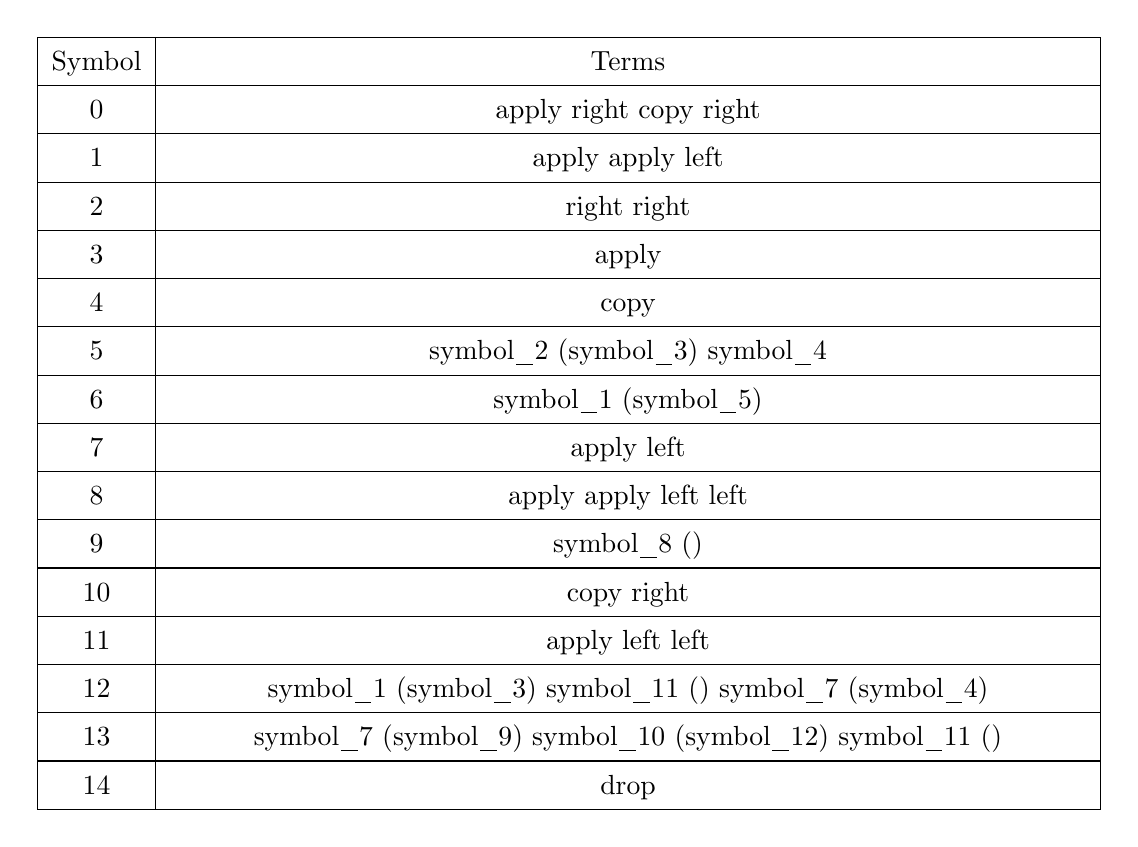
\begin{tikzpicture}[cell/.style={rectangle,draw=black},
space/.style={
        minimum height=1.5em,matrix of nodes,row sep=-\pgflinewidth,column sep=-\pgflinewidth,
        column 1/.style={font=\ttfamily}
    },
    text depth=0.5ex,text height=2ex,nodes in empty cells]

\matrix (first) [space, 
    column 1/.style={nodes={cell, minimum width=1.5cm}},
    column 2/.style={nodes={cell, minimum width=12cm}}
] {
Symbol   & Terms \\
0   & apply right copy right \\
1   & apply apply left \\  
2   & right right \\  
3   & apply \\  
4   & copy \\  
5   & symbol\_2 (symbol\_3) symbol\_4 \\  
6   & symbol\_1 (symbol\_5) \\  
7   & apply left \\  
8   & apply apply left left \\  
9   & symbol\_8 () \\  
10   & copy right  \\  
11   & apply left left \\  
12   & symbol\_1 (symbol\_3) symbol\_11 () symbol\_7 (symbol\_4) \\   
13   & symbol\_7 (symbol\_9) symbol\_10 (symbol\_12) symbol\_11 () \\   
14   & drop \\  
};

\end{tikzpicture}
    \caption{Kihi Intermediary Representation}
    \label{fig:kihi_intermediary_representation}
\end{figure}

\subsection{Symbolic Analysis}
\todo[inline]{Find reference probably simmilar idea exists in lit}
The Kihi virtual machine implements a relatively simple symbol analyser.
The base symbolic analyser combines adjacent operators into symbols. The
motivation behind this method

\section{Execution Style}


\section{Benchmark Suite}

\begin{figure}[htb]
    \centering
    \begin{lstlisting}
execute_program(input: String):
    terms: []Term := parse_program(input)
    
    reductible_term: Index := find_reductible_term(terms)
    while (reductible_term != -1) {
        reduce_term(terms, reductible_term)
    }

find_reductible_term(terms: []Term):
    for i: Index in 0..|terms| {
        if terms[i] is 'apply'
            and terms[i+1] is abstraction => return i
        else if terms[i] is 'left'
            and terms[i+1] and terms[i+2] are abstractions => return i
        else if terms[i] is 'drop'
            and terms[i+1] => return i
        ... and so on for each inference rule
        }
    }
    return -1

reduce_term(terms: []Term, term: Index):
    if terms[index] is 'apply'
        terms[index..index+1] = terms[index+1]
    else if terms[index] is 'left'
        terms[index..index+2] = [terms[index+2], ...terms[index+1]]
    else if terms[index] is 'drop'
        terms[index..index+1] = []
    ... and so on for each inference rule
    \end{lstlisting}
    \caption{Pseudocode for a term rewriting based Kihi implementation}
    \label{fig:term_rewriting_pseudocode}
\end{figure}
\begin{figure}[htb]
    \centering
    \begin{lstlisting}
execute_program(input: String):
    program: []Term := parse_program(input)
    
    stack: []Term := []
    
    while(|terms| != 0) {
        term := terms.pop()
        if term is abstraction => stack.push(term)
        else if term is 'apply' => program.append( stack.pop() )
        else if term is 'left' => {
            arg1 = stack.pop()
            arg2 = stack.pop()
            stack.push( [arg2] ++ arg2 )
        }
        ... and so on for each inference rule
    }
    \end{lstlisting}
    \caption{Pseudocode for a stack based Kihi execution}
    \label{fig:stack_pseudocode}
\end{figure}
\chapter{Results and Evaluation} \label{C:results}

\section{Method}


\begin{figure}[htb]
    \centering
    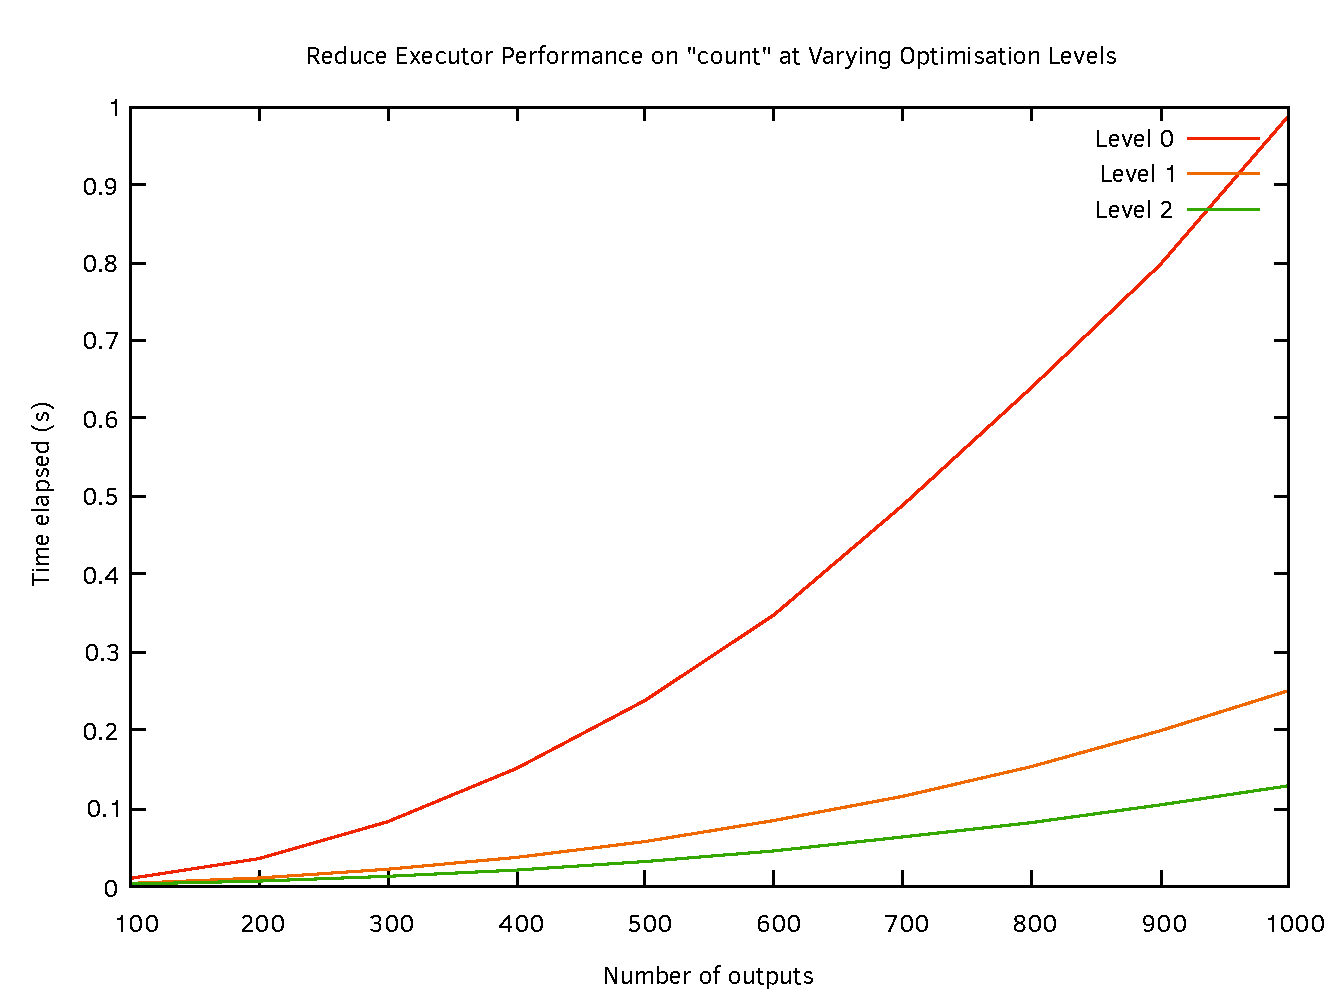
\includegraphics[width=\textwidth]{reduce_executor_fig_1}
    \caption{A chart demonstrating the effect of varying optimisations}
    \label{fig:reduce_executor_performance_on_count}
\end{figure}


Figure \ref{fig:reduce_executor_performance_on_count} shows the effects of the various optimisations on program performance. level 0 represents a baseline state without any optimisations.

\todo[inline]{Put results here}
\todo[inline]{Merge results and evaluation?}
\chapter{Implementation} \label{C:implementation} 

\section{Execution Style}
There are two main execution styles that can be used to execute
a Kihi program: a term rewriting approach and a stack based 
approach. These two approachs are identical for side-effect
free and terminating programs, however, the observed
behaviour for other varieties of programs can differ
substantially depending on the execution style. The rest of 
this section describes these two execution styles and 
concludes by contrasting their behaviour.

\subsubsection{Term Rewriting}
Term rewriting is the process of finding
and replacing reducible terms with their reduced form. For Kihi,
this means finding terms which are directly followed by
some number of abstractions. The specific number of abstractions
required is determined by the term and can be thought of as the
number of arguments. This execution paradigm allows execution
to occur anywhere in the program because a reducible term may
be found anywhere in the program and this reduction can be
thought of as an execution step.

\subsubsection{Stack Based}
Stack based execution imagines the terms of the program as
instructions for a stack machine. The terms are scanned
right to left and an action performed depending on the term
encountered. For instance, whenever an abstraction is found
it is pushed onto the stack and whenever a drop is found the
topmost value of the stack is popped and discarded.

\subsubsection{Differences}
A term rewriting based virtual machine will be able to execute
all programs a stack based machine is able to. The proof of this
is relatively simple. One can imagine a term rewriting machine 
that searches for reducible terms right to left as equivilent to
a stack machine for terminating programs.

A program representing an infinite data structure, such as the count
program which outputs a continous stream of numbers, cannot be
processed through a normal stack based approach. There may be alterations
to the stack based approach which may allow values to be pushed 
through to the left hand side of the program.


an abstraction is
encountered it is pushed onto the stack and when a term (reword)
is found the arguments are popped off the stack and the 
result, if it is an abstraction, is pushed onto the stack.

The first approach involves finding and replacing
reducible terms with their reduced form. The essence of this
execution style is shown in figure 
\ref{fig:term_rewriting_pseudocode} which provides a pseudocode
description of the essential algorithm.

These two different approaches are identical for
terminating programs but can display very different behaviour
for non-terminating programs.
Any acknowledgments should go 
in here, between the title page and the table of contents.  The 
acknowledgments do not form a proper chapter, and so don't get a 
number or appear in the table of contents.

\chapter{Conclusions}\label{C:con}
The conclusions are presented in this Chapter.




%%%%%%%%%%%%%%%%%%%%%%%%%%%%%%%%%%%%%%%%%%%%%%%%%%%%%%%

\backmatter

%%%%%%%%%%%%%%%%%%%%%%%%%%%%%%%%%%%%%%%%%%%%%%%%%%%%%%%


%\bibliographystyle{ieeetr}
\nocite{*}
\bibliographystyle{acm}
\bibliography{bib/bib}


\end{document}
